
%%%%%%%%%%%%%%%%%%%%%%%%%%%%%%%%%%%%%%%%%%%%%%%%%%%%%%%%%%%%%%%%%%%%
%% I, the copyright holder of this work, release this work into the
%% public domain. This applies worldwide. In some countries this may
%% not be legally possible; if so: I grant anyone the right to use
%% this work for any purpose, without any conditions, unless such
%% conditions are required by law.
%%%%%%%%%%%%%%%%%%%%%%%%%%%%%%%%%%%%%%%%%%%%%%%%%%%%%%%%%%%%%%%%%%%%

\documentclass[compress]{beamer}
\usetheme[faculty=phil, navigation, microtype]{fibeamer}
%\usetheme[logo=resources/NOKIA]{fibeamer}
\useoutertheme{miniframes}
\setbeamercolor{section in head/foot}{fg=white, bg=fibeamer@blue}
\usepackage[francais]{babel}
\usepackage[utf8]{inputenc}
\usepackage[T1]{fontenc}
%\title{Requêtes probabilistes et pondérées en logique d'arbre de calcul %
\includegraphics[width=0.25\linewidth]{fibeamer/logo/mu/storm}
\title{Vérification des Processus Décisionnels de Markov pondérés
} %% that will be typeset on the
%\subtitle{Presentation Subtitle} %% title page.
\author{Florent Delgrange}
\vspace{0.5cm}
\subtitle{\normalsize UMONS \\ Faculté des Sciences \\ Mab2 Science Informatique}
\date{\today}
%% These additional packages are used within the document:
\usepackage{ragged2e}  % `\justifying` text
\usepackage{bbold}
\usepackage{booktabs}  % Tables
\usepackage{centernot}
\usepackage{tabularx}
\usepackage{tikz}      % Diagrams
\usetikzlibrary{calc, shapes, backgrounds}
\usepackage{arevtext,arevmath}
\usepackage{verbatim}
\usepackage{amsmath, amssymb}
\usepackage{url}       % `\url`s
\usepackage{listings}
\usepackage{changepage}
\usepackage{cprotect}
\usepackage{caption}
\usepackage{graphicx}
\usepackage{minted}
\usepackage{biblatex}
\usepackage{mathtools}
\usepackage{multicol}
\frenchspacing

%% PRISM CODE LISTING *********************************************

\definecolor{prismgreen}{rgb}{0, 0.6, 0}

\lstdefinelanguage{Prism}{ % syntax highlight via font
	basicstyle=\color{red}\tiny\ttfamily, % small true type font (like courier)
	keywords=
	{bool,C,ceil,const,ctmc,double,dtmc,endinit,endmodule,endrewards, endsystem,F,false,floor,formula,G,global,I,init,int,label,max,mdp,min,
	module,nondeterministic,P,Pmin,Pmax,prob,probabilistic,R,rate,rewards, Rmin,Rmax,S,stochastic,system,true,U,X},
	keywordstyle={\bfseries\color{black}},
	numberstyle=\tiny\color{black},
	comment=[l] {//}, morecomment=[s]{/*}{*/}, % single and multi-line
	commentstyle= \color{prismgreen}, % dark green
	tabsize=4, % tab treatment (going to be fixed in Prism)
	captionpos=b, % put captions at the bottom
	escapechar=@ % write LaTeX comments escaped by @ symbol
}

%define command \prism with one argument for inline printing of \prism code
\newcommand{\prism}[1]{\lstinline[language=Prism,basicstyle=\small
	\ttfamily]|#1|}

%% END PRISM CODE LISTING


\newtheorem*{exemple}{Exemple}

\definecolor{DarkOrange}{HTML}{FF8C00}

\bibliography{bib}
\begin{document}
  \begin{frame}[plain]
    \maketitle
  \end{frame}

  \AtBeginSection[]
    {
      %  \begin{frame}<beamer>
      %  \frametitle{Plan}
      %  \tableofcontents[currentsection]
      %  \end{frame}
      \begin{frame}{\contentsname}
      \vspace{-0.05\linewidth}
      \footnotesize
      \begin{multicols}{2}
      \tableofcontents[currentsection]
      \end{multicols}
      \end{frame}
    }

\section{Préliminaires}
\subsection{Système de transition}
\begin{frame}{Système de transition}
\begin{definition}[Système de transition]
Un \textit{système de transition} (noté TS, pour \textit{transition system}) est un tuple $\mathcal{T} = (S, A, \rightarrow, AP, L)$ où
\begin{itemize}
  \item $S$ est un ensemble d'états,
  \item $A$ est un ensemble d'actions,
  \item $\rightarrow \subseteq S \times A \times S$ est une relation de transition,
  \item $AP$ est un ensemble de propositions atomiques et
  \item $L: S \rightarrow 2^{AP}$ est une fonction d'étiquetage.
\end{itemize}
\end{definition}
\end{frame}

\begin{frame}{Système de Transition}
  \begin{itemize}
    \item \textbf{\color{fibeamer@orange}Idée} : Graphe orienté
      \begin{itemize}
        \item noeuds : états du système
        \item arcs : transitions du système
      \end{itemize}
    \item \textbf{\color{fibeamer@orange}\'Etat}: décrit les informations d'un système à un certain moment de son comportement.
    \item \textbf{\color{fibeamer@orange}Transition}: si un état a plus d'une transition sortante, alors le comportement du système est \alert {non-déterministe}, i.e., l'évolution du système requiert la sélection d'une transition.
    \item \textbf{\color{fibeamer@orange}\'Etiquetage}: $L(s)$ est l'ensemble des étiquettes $a \in AP$ de l'état $s$.
    \item \textbf{\color{fibeamer@orange}Pas d'états terminaux !}
  \end{itemize}
\end{frame}


\begin{frame}{Système de Transition}{Exemple}
    \centering
    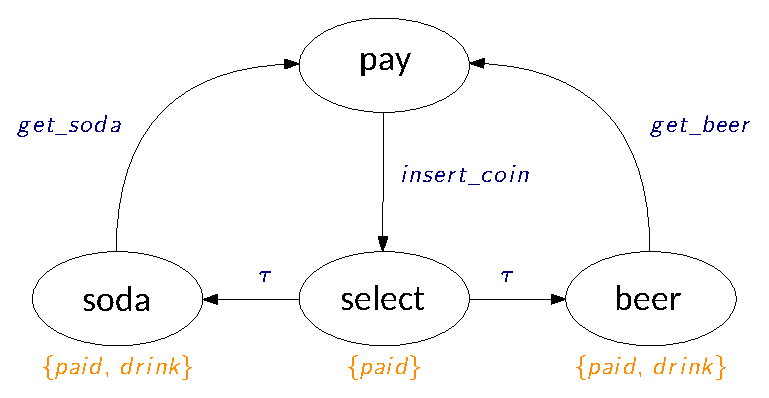
\includegraphics[width=0.7\linewidth]{resources/TS.eps}
    \captionof{figure}{Distributeur de boissons \protect \cite{PMC}}% \protect \cite{DBLP:books/daglib/0020348}}
    \scriptsize
    \begin{columns}
      \begin{column}{0.65\textwidth}
        \begin{itemize}
          \item $ S = \{ pay, \, select, \, beer, \, soda \}$
          \item $ A = \{ insert\_coin,\, \tau,\, get\_soda,\, get\_beer\}$
        \end{itemize}
      \end{column}
      \begin{column}{0.35\textwidth}
        \begin{itemize}
          \item $AP = \{ paid, \, drink \}$
        \end{itemize}
      \end{column}
    \end{columns}
\end{frame}

\subsection{Chemins et Traces de TS}
\begin{frame}{Chemins}
Un chemin d'un système de transition est une succession d'état possible résultant de l'exécution de ce système.
\begin{itemize}
  \item \textbf{\color{fibeamer@orange}Idée}: pas d'états terminaux $\implies$
    chemins infinis.
\end{itemize}
\begin{definition}[Chemin d'un TS]
  Soit $\mathcal{T} = (S, A, \rightarrow, AP, L)$, un TS. \\
  $\pi = s_0 s_1 s_2 s_3 \dots$ est un \textit{chemin} (infini) de $\mathcal{T}$ ssi
  pour tout $i \in \mathbb{N}$, il existe une action $\alpha \in A$ telle que
  $s_i \xrightarrow{\alpha} s_{i+1}$, avec $s_i, s_{i+1} \in S$% et $(s_i, \alpha, s_{i+1}) \in \rightarrow$
  . \\
  L'ensemble des chemins (infinis) $\pi = s_0s_1\dots$ commençant en l'état $s$ (i.e., tels que $s_0 = s$) est dénoté par $Paths(s)$.

\end{definition}

\end{frame}

\begin{frame}{Traces}
    Les traces d'un système de transition sont des mots infinis sur l'alphabet $2^{AP}$ formés lors de l'exécution du système. \\
\begin{definition}[Traces]
  Soit $\mathcal{T} = (S, A, \rightarrow, AP, L)$, un TS. La trace du chemin $\pi = s_0s_1 \dots$ est donné par \[trace(\pi) = L(s_0)L(s_1)\dots\]
  Dès lors, soit $s \in S$, un état de $\mathcal{T}$, les traces du système
  provenant de l'état $s$ est donné par \[Traces(s) = \{ trace(\pi) \; | \; \pi \in
  Paths(s) \}\]
\end{definition}
\end{frame}

\begin{frame}{Chemins et Traces}{Exemple}
    \centering
    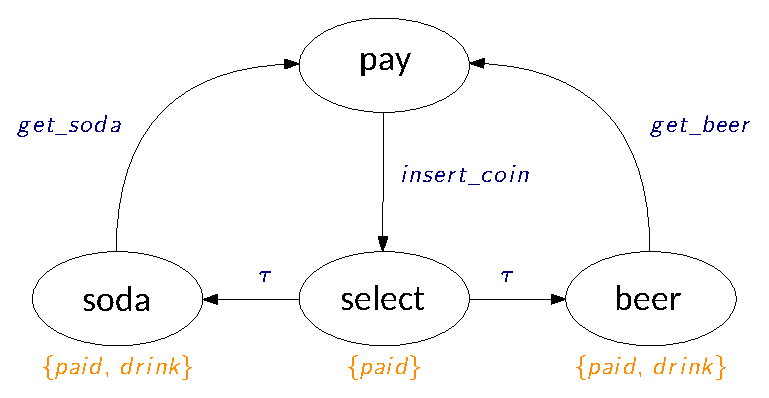
\includegraphics[width=0.7\linewidth]{resources/TS.eps}
    \captionof{figure}{Distributeur de boissons \protect \cite{PMC}}% \protect \cite{DBLP:books/daglib/0020348}}
    \scriptsize
    \begin{itemize}
      \item $\pi = pay\; select \; soda \; pay \; select \; beer \; \dots \in Paths(pay)$
      \item $\emptyset\{paid\}\{paid, \, drink\}\emptyset\{paid\}\{paid, \, drink\} \dots = trace(\pi) \in Traces(paid)$
    \end{itemize}
\end{frame}

\section{LTL}
\subsection{Intuition}
\begin{frame}{Logique temporelle linéaire (LTL)}
\begin{itemize}
  \item L'exactitude des systèmes réactifs dépend des exécutions + de l'équité du système
  \item La logique {\color{fibeamer@orange}temporelle} permet de traiter ces aspects
  \begin{itemize}
    \item[$\rightarrow$] \textit{temps ``réel''} (discret!)
  \end{itemize}
  \item Temps linéaire $\implies$ logique basée sur les {\color{fibeamer@orange}chemins du système}
    \begin{itemize}
      \item[$\rightarrow$] \`a chaque étape, un seul successeur est possible
    \end{itemize}
    \item[$\rightarrow$] \textbf{\color{fibeamer@orange}LTL} $\approx$ langage qui a pour but de vérifier des propriétés sur les exécutions d'un système% à l'aide d'{\color{fibeamer@orange}opérateurs temporels}
\end{itemize}
\end{frame}

\begin{frame}{Logique temporelle linéaire (LTL) : intuition}
  \vspace{-0.04\linewidth}
  \footnotesize
  Soit $\mathcal{T} = (S, A, \rightarrow, AP, L)$,
  LTL est formée par ...
  \begin{enumerate}
    \item des propositions atomiques $a \in AP$,
    \item des combinaisons booléennes de formules :
    $
      \neg \phi, \; \phi \wedge \psi, \, \phi \vee \psi
    $
     et
    \item des opérateurs temporels : soit $\pi = s_0s_1s_2s_3\dots \in Paths(\mathcal{T})$
    \begin{center}
      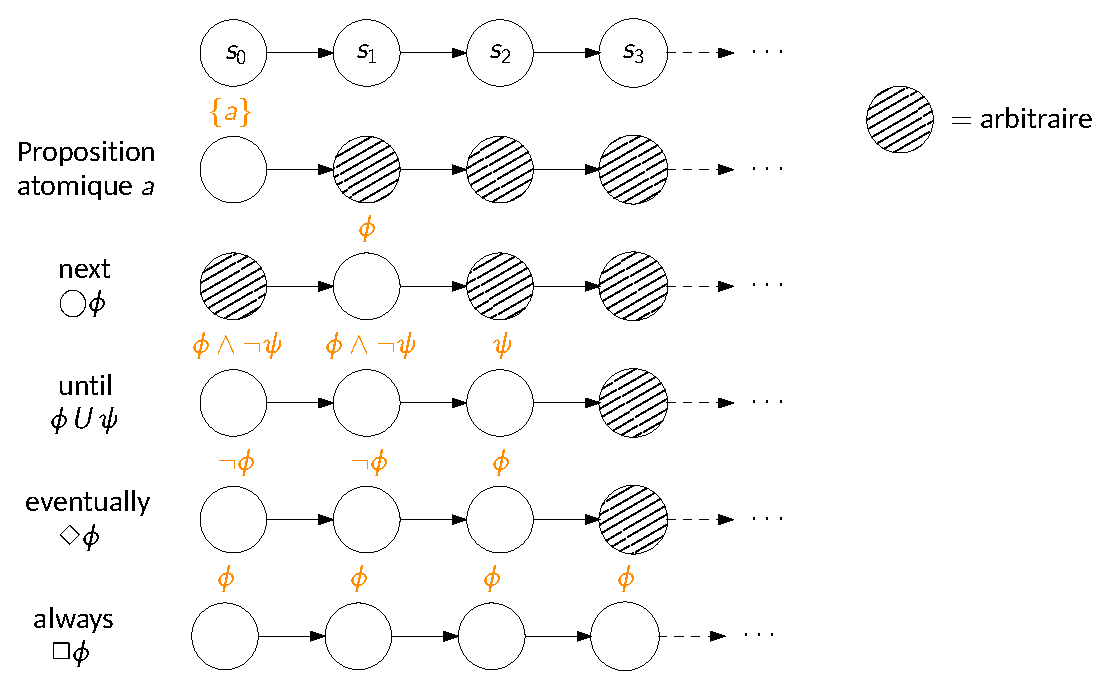
\includegraphics[width=0.8\linewidth]{resources/LTL}
    \end{center}
  \end{enumerate}
\end{frame}

\subsection{Syntaxe}
\begin{frame}
\begin{block}{Syntaxe}
Soit $AP$, un ensemble de propositions atomiques, les \textit{\color{fibeamer@orange}formules} LTL sont formées selon la {\color{fibeamer@orange}grammaire} suivante :
\[
  \phi ::= true \; | \; a \; | \; \phi \wedge \psi \; | \; \neg \phi \; | \; \bigcirc \phi \; | \; \phi U \psi
\]
où $a \in AP$
\end{block}
  \alert{Note : $\phi U \psi$ requiert l'apparition de $\psi$ dans le chemin; $\phi$ indéfiniment n'est pas suffisant !}

\end{frame}

\begin{frame}{Syntaxe}{}
\vspace{-0.05\linewidth}
{\color{fibeamer@orange}Opérateurs dérivés : \\ }
\vspace{-0.03\linewidth}
\begin{columns}
  \begin{column}{0.3\linewidth}
    eventually\\
    always \\
  \end{column}
  \begin{column}{0.3\linewidth}
    $ \Diamond \phi \equiv true\, U\, \psi$ \\
    $ \Box \phi \equiv \neg \Diamond \neg \phi $ \\
  \end{column}
\end{columns}
{\vspace{0.02\linewidth}\color{fibeamer@orange}Ordre de précédence: \\ }
\vspace{-0.05\linewidth}
\begin{enumerate}
  \item parenthèses
  \item opérations unaires $\big(\, \neg, \, \bigcirc\, \big)$
  \item opérations binaires :
    \begin{enumerate}
      \item $U \; \big($assosiatif par la droite,
      e.g., $\phi_1 U \phi_2 U \phi_3 \equiv \phi_1 U (\phi_2 U \phi_3) \, \big)$
      \item $\wedge$
    \end{enumerate}
\end{enumerate}
{\color{fibeamer@orange}Combinaisons de modalités temporelles :}
\begin{itemize}
  \item $\Box\Diamond \phi \quad \quad $ ``infiniment souvent $\phi$''
  \item $\Diamond\Box \phi \quad \quad $ ``éventuellement toujours $\phi$''
\end{itemize}
\end{frame}

\begin{frame}{Combinaisons de modalités temporelles}{Exemple (infiniment souvent)}
    \centering
    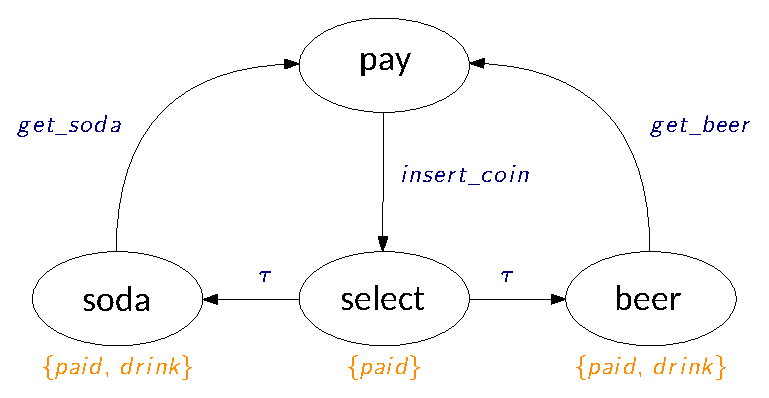
\includegraphics[width=0.7\linewidth]{resources/TS.eps}
    \captionof{figure}{Distributeur de boissons \protect \cite{PMC}}% \protect \cite{DBLP:books/daglib/0020348}}
    \begin{itemize}
      \item Pour toute trace de l'éxécution du système depuis $pay$, i.e., $\forall \sigma \in
        Traces(pay)$, pour toute position dans $\sigma$, le label $drink$ doit apparaître dans le futur. \\
      $\leadsto \Box\Diamond drink$
    \end{itemize}
\end{frame}

\begin{frame}{Combinaisons de modalités temporelles}{Exemple (éventuellement toujours)}
  \centering
  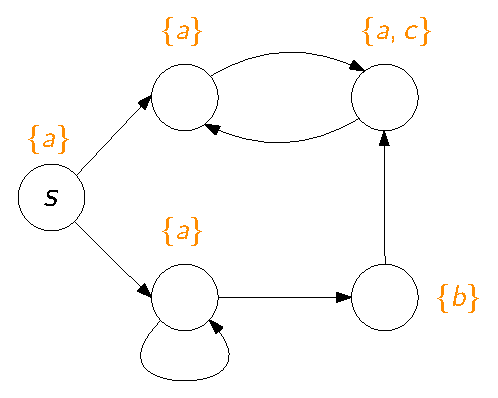
\includegraphics[width=0.45\linewidth]{resources/LTL_example2}
    \captionof{figure}{\protect \cite{MRV}}% \protect \cite{DBLP:books/daglib/0020348}}
  \begin{itemize}
    \item $\forall \sigma \in Traces(s)$, il y a toujours un moment où on voit toujours $a$, mais plus $b$ \\
    $\leadsto \Diamond\Box(a \wedge \neg b)$
  \end{itemize}
\end{frame}

\subsection{Sémantique}
\begin{frame}{Sémantique}
\small
Soient $\mathcal{T} = (S, A, \rightarrow, AP, L)$ et $\phi$, une formule LTL sur $AP$, la propriété LT induite par $\phi$ est le langage de mots
\[
  Words(\phi) = \{ \sigma = A_0A_1A_2\dots \in (2^{AP})^\omega \; | \; \sigma \models \phi \}
\]
où $\models$ est la plus petite relation satisfaisant
\begin{align*}
  & \sigma \models true &&& \\
  & \sigma \models a && \text{ssi } a \in A_0& \\
  & \sigma \models \phi \wedge \psi && \text{ssi } \sigma \models \phi \text{ et } \sigma \models \psi& \\
  & \sigma \models \neg\phi && \text{ssi } \sigma \not\models \phi&\\
  & \sigma \models \bigcirc \, \phi && \text{ssi } \sigma[1:] = A_1A_2\dots \models \phi&\\
  & \sigma \models \phi U \psi && \text{ssi } \exists j \geq 0, \; \sigma[j:] \models \psi \text{ et } \forall 0 \leq i < j, \; \sigma[i:] \models \phi
\end{align*}
\end{frame}

\begin{frame}{Sémantique}
\small
Soit $s \in S$,
\begin{itemize}
  \item $\forall \pi \in Paths(s)$, $\pi \models \phi$ ssi $trace(\pi) \models \phi$
  \item $s \models \phi$ ssi $\forall \pi \in Paths(s)$, $\pi \models \phi$
\end{itemize}

\textit{\color{gray}Exemple}
\vspace{-0.02\linewidth}
\begin{center}
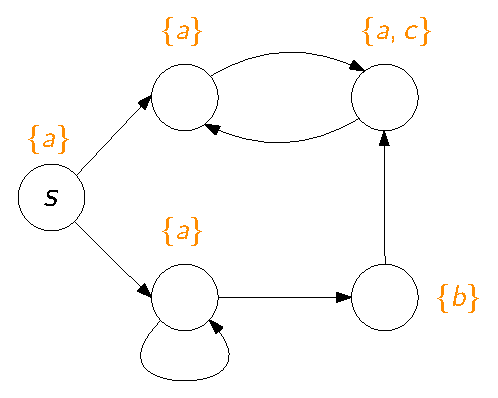
\includegraphics[width=0.4\linewidth]{resources/LTL_example2}
\captionof{figure}{\protect \cite{MRV}}% \protect \cite{DBLP:books/daglib/0020348}}
\end{center}
\begin{itemize}
  \item $s \models \Diamond\Box (a \wedge \neg b)$
\end{itemize}
\end{frame}

\section{CTL}
\subsection{Intuition}

\begin{frame}{Logique d'arbre de calculs (CTL)}
\begin{itemize}
  \item Notion d'\textbf{\color{fibeamer@orange}arbre d'exécution = arbre de calcul}
  \item[$\leadsto$] Dépliage infini du système considérant toutes les possibilités de branchement
\end{itemize}
\end{frame}

\begin{frame}{Arbre de calculs}
\small
\begin{center}
  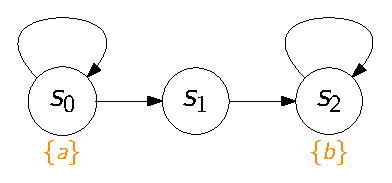
\includegraphics[width=0.35\linewidth]{resources/CTL_unfolding1}
\end{center}
  Arbre de calculs depuis l'état $s_0$ ? \\
\begin{columns}
\begin{column}{0.6\linewidth}
  \centering
  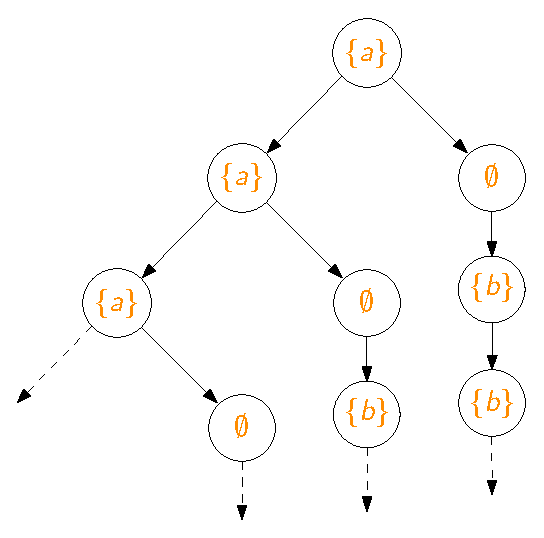
\includegraphics[width=0.6\linewidth]{resources/CTL_unfolding2}
\end{column}
\begin{column}{0.5\linewidth}
  Est-ce que toutes les exécutions ont toujours la possibilité d'atteindre
  éventuellement {\color{DarkOrange}$\{b\}$} ? \\
  %$\rightarrow$ \alert{non}
\end{column}
\end{columns}
\end{frame}

\begin{frame}{Quantificateurs}
\begin{itemize}
  \item \textbf{\color{fibeamer@orange}LTL} : $s\models\phi$ signifie que tous les chemins commençant en $s$ satisfont $\phi$
  \begin{itemize}
    \item Quantification explicite !
    \item $s \models \forall \phi$
  \end{itemize}
  \item \textbf{\color{fibeamer@orange}CTL} : on peut considérer seulement certains chemins
  \begin{itemize}
    \item Existe-t-il un chemin satisfaisant $\phi$ commençant en $s$ ?
    \item $s \models \exists \phi \iff \underbrace{s \not\models \forall \neg \phi}_{\text{LTL : }s \not \models \neg \phi}$
  \end{itemize}
\end{itemize}
\end{frame}

\begin{frame}{Quantificateurs}{Motivation}
\small
\begin{columns}
\begin{column}{0.6\linewidth}
  \centering
  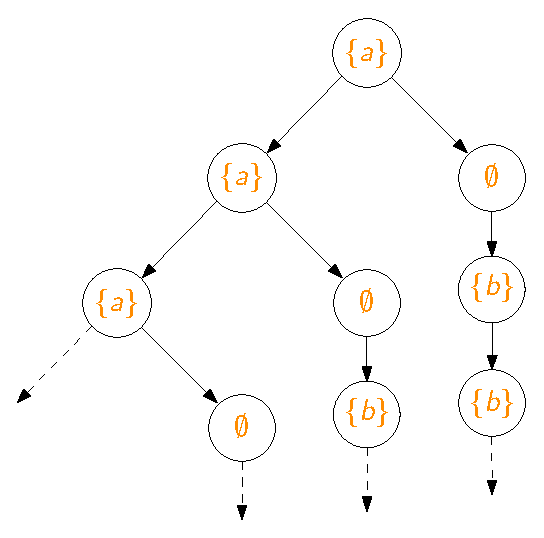
\includegraphics[width=0.6\linewidth]{resources/CTL_unfolding2}
\end{column}
\begin{column}{0.5\linewidth}
  Est-ce que \alert{toutes} les exécutions ont toujours \alert{la possibilité} d'atteindre
  éventuellement {\color{DarkOrange}$\{b\}$} ? \\
  %$\rightarrow$ \alert{non}
\end{column}
\end{columns}
\begin{itemize}
  \item \textbf{\color{fibeamer@orange}LTL} :
  \begin{itemize}
    \item $s_0 \models \Box\Diamond b$ \alert{ne fonctionne pas !}
    \item requiert que \alert{tous les chemins du système de transition} atteignent
      {\color{DarkOrange}$\{b\}$}
    \item[$\leadsto$] On ne parle pas de possibilité d'atteindre
      {\color{DarkOrange}$\{b\}$}
  \end{itemize}
  \alert{
  \item Pas expressible en LTL
  }
\end{itemize}
\end{frame}

\begin{frame}{Quantificateurs}{Motivation}
\small
\begin{columns}
\begin{column}{0.6\linewidth}
  \centering
  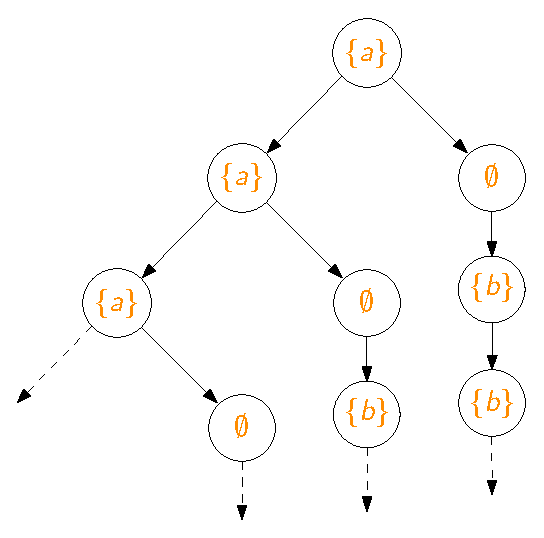
\includegraphics[width=0.6\linewidth]{resources/CTL_unfolding2}
\end{column}
\begin{column}{0.5\linewidth}
  Est-ce que \alert{toutes} les exécutions ont toujours \alert{la possibilité} d'atteindre
  éventuellement {\color{DarkOrange}$\{b\}$} ? \\
  %$\rightarrow$ \alert{non}
\end{column}
\end{columns}
\begin{itemize}
  \item[$\rightarrow$] Besoin de quantificateurs
  \item \textbf{\color{fibeamer@orange}CTL} :
  \begin{itemize}
    \item $s_0 \models \forall\Box\exists\Diamond b$
    \item Pour tout chemin commençant en $s_0$, à chaque étape, il existe un chemin qui peut atteindre $b$.
  \end{itemize}
\end{itemize}
\end{frame}

\begin{frame}{CTL vs LTL}{Comparaison intuitive}
  \begin{itemize}
    \item \textbf{\color{fibeamer@orange}LTL : }
    \begin{itemize}
      \item chemins + traces
      \item temps linéaire
      \item chaque point a un seul futur possible
    \end{itemize}
    \item \textbf{\color{fibeamer@orange}CTL : }
    \begin{itemize}
      \item arbre de calculs + comportement des branchements
      \item temps en branchements
      \item chaque noeud de l'arbre a plusieurs futurs possibles
    \end{itemize}
  \end{itemize}
\end{frame}

\begin{frame}{CTL}{Intuition}
\begin{itemize}
  \item Formules d'états
  \item[=] Assertions de propositions atomiques dans des états ainsi que leur structure de branchement
  \begin{itemize}
    \item propositions atomiques $a \in AP$
    \item combinaisons booléennes de formules :
      $\neg \Phi, \, \Phi \wedge \Psi, \, \Phi \vee \Psi$
    \item quantification de chemins via des {\color{fibeamer@orange} formules de chemins}
  \end{itemize}
\end{itemize}
\end{frame}

\begin{frame}{CTL}{Intuition}
\vspace{-0.05\linewidth}
\begin{itemize}
  \item Formules de chemins \\
\end{itemize}
\vspace{0.05\linewidth}
\centering
\begin{columns}
  \begin{column}{0.5\linewidth}
    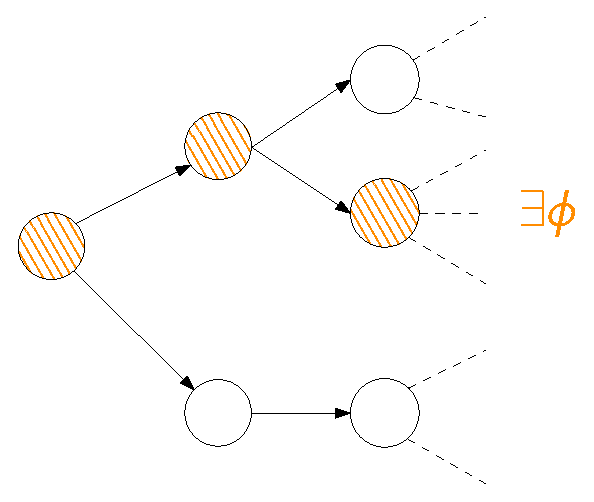
\includegraphics[width=\linewidth]{resources/ctl_path_formulae}
  \end{column}
  \begin{column}{0.5\linewidth}
    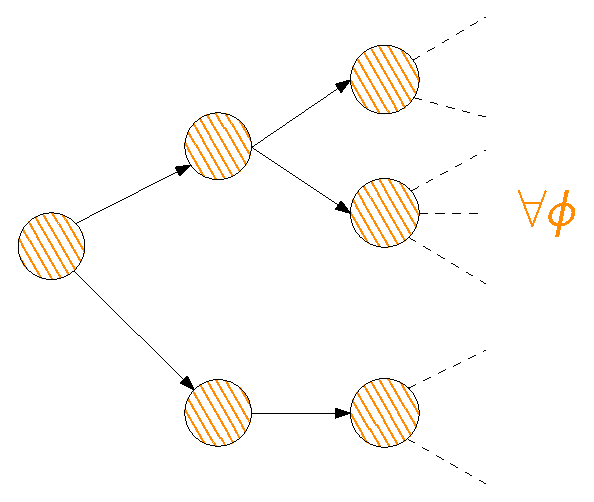
\includegraphics[width=\linewidth]{resources/ctl_path_formulae2}
  \end{column}
\end{columns}
\end{frame}

\begin{frame}{Formules de chemins}
  Formules LTL $\neq$ formules de chemin CTL ! \\
  En effet, les formules de chemin CTL...
  \begin{itemize}
    \item ne peuvent pas être combinées avec des connecteurs booléens
    \item ne permettent pas l'imbrication des modalités temporelles \\
    \textit{\color{gray}Exemple : }\\
    \begin{align*}
      &s \models \forall \Box\exists\Diamond b && \text{\color{green}correct}& \\
      &s \models \forall \Box\Diamond b && \text{\alert{incorrect}}&
    \end{align*}
  \end{itemize}
\end{frame}

\subsection{Syntaxe}
\begin{frame}
  \begin{block}{Syntaxe}
    Soit $AP$, un ensemble de propositions atomiques.
    \begin{itemize}
      \item Les \textit{\color{fibeamer@orange}formules d'états} CTL sont formées selon la
    grammaire suivante :
    \[
      \Phi ::= true \; | \; a \; | \; \Phi \wedge \Psi \; | \; \neg \Phi \; | \; \exists \phi \; | \; \forall \phi
    \]
    où $a \in AP$ et $\phi$ est une formule de chemin.
      \item Les \textit{\color{fibeamer@orange}formules de chemins} CTL sont formées selon la grammaire suivante :
      \[
        \phi ::= \bigcirc\,\Phi \; | \; \Phi U \Psi
      \]
      où $\Phi$ et $\Psi$ sont des formules d'états.
    \end{itemize}
  \end{block}
\end{frame}

\subsection{Sémantique}
\begin{frame}{Sémantique}
  Soient $\mathcal{T} = (S, A, \rightarrow, AP, L)$, un TS et $s \in S$, un {\color{fibeamer@orange}état}
  de $\mathcal{T}$. \\
  $s \models \Phi$ ssi la formule $\Phi$ tient dans l'état $s$, i.e.,
  \begin{align*}
    &s \models true &&&\\
    &s \models a &\text{ ssi }& a \text{ est un label de $s$, i.e., } a \in L(s)&\\
    &s \models \Phi \wedge \Psi&\text{ ssi }& s \models \Phi \text{ et } s \models \Psi&\\
    &s \models \neg \Phi &\text{ ssi }& s \not\models \Phi&\\
    &s \models \exists \phi &\text{ ssi }& \exists \pi \in Paths(s), \, \pi \models \phi&\\
    &s \models \forall \phi &\text{ ssi }& \forall \pi \in Paths(s), \, \pi \models \phi&
  \end{align*}
\end{frame}

\begin{frame}{Sémantique}
  Soient $\mathcal{T} = (S, A, \rightarrow, AP, L)$, un TS et $\pi = s_0s_1s_2\dots \in Paths(s)$, un {\color{fibeamer@orange}chemin}.\\
  $\pi \models \phi$ ssi $\pi$ satisfait $\phi$, i.e.,
  \begin{align*}
  &\pi \models \Phi&\text{ ssi }&s_0 \models \Phi&\\
  &\pi \models \bigcirc\, \Phi&\text{ ssi }&s_1 \models \Phi&\\
  &\pi \models \Phi U \Psi &\text{ ssi }& \exists j \in \mathbb{N},\, s_j \models \Psi
    \text{ et } \forall 0 \leq i < j, \, s_i \models \Phi&\\
  & \pi \models \Diamond \Phi&\text{ ssi }& \exists j \in \mathbb{N}, \, s_j \models \Phi&\\
  & \pi \models \Box \Phi&\text{ ssi }& \forall j \in \mathbb{N}, \, s_j \models \Phi&
  \end{align*}
\end{frame}

%\subsection{Satisfiabilité}

\begin{frame}{Satisfiabilité}
  \begin{definition}[Ensemble de satisfaction]
    Soient $\mathcal{T} = (S, A, \rightarrow, AP, L)$, un TS et
    $\Phi$, une formule d'état CTL sur $AP$. L'ensemble
    de satisfaction du TS $\mathcal{T}$ est donné par
    \[
      Sat_\mathcal{T}(\Phi) = \{s \in S \; | \; s \models \Phi \}
    \]
  \end{definition}
\end{frame}

% \begin{frame}{Caractérisation de Sat}
%   Soient $\mathcal{T}=(S, A, \rightarrow, AP, L)$, un TS et les formules d'états CTL $\Phi$, $\Psi$ sur $AP$.
%   \begin{itemize}
%     \item $Sat_\mathcal{T}(true)=S$
%     \item $Sat_\mathcal{T}(a) = \{s \in S \; | \; a \in L(s)\}$, avec $a \in AP$
%     \item $Sat_\mathcal{T}(\Phi \wedge \Psi) = Sat_\mathcal{T}(\Phi) \cap Sat_\mathcal{T}(\Psi)$
%     \item $Sat_\mathcal{T}(\neg \Phi) = S \setminus Sat_\mathcal{T}(\Phi)$
%     \item $Sat_\mathcal{T}(\exists \bigcirc \Phi) = \{ s \in S \; | \; Succ(s) \cap Sat_\mathcal{T}(\Phi) \neq \emptyset \}$
%   \end{itemize}
% \end{frame}

\subsection{LTL vs CTL}
\begin{frame}{LTL vs CTL}
\textbf{\alert{\large LTL et CTL sont incomparables !}} \\
\textit{Exprimable en ...}
\begin{itemize}
  \item CTL mais pas LTL :\\
    $\forall\Box\exists\Diamond a$ {\color{gray}(voir exemple)}
  \item LTL mais pas CTL : \\
  $\Diamond\Box a$
\end{itemize}
En effet, \alert{$\Diamond\Box a \not \equiv \forall \Diamond \forall \Box a$ !}
\begin{itemize}
  \item $\Diamond\Box a$ assure que $a$ sera atteint éventuellement en tout point.
  \item $\forall\Diamond\forall\Box a$ affirme que pour toute exécution, un état
    $s$ est éventuellement atteint, tel que $s \models \forall \Box a$
\end{itemize}
\end{frame}

\begin{frame}{LTL vs CTL}{Exemple}
\vspace{-0.05\linewidth}
\begin{itemize}
  \item AP = {\color{DarkOrange}$\{a\}$}
\end{itemize}
\begin{center}
  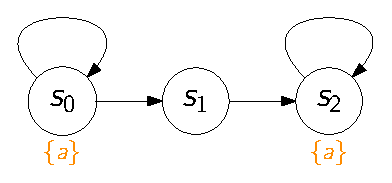
\includegraphics[width=0.4\linewidth]{resources/ctl_vs_ltl}
\end{center}
\vspace{-0.05\linewidth}
\begin{itemize}
  \item $s_0$ satisfait la formule LTL $\Diamond \Box a$ car
  chaque chemin commençant en $s_0$ reste éventuellement toujours en $s_0$ ou en
  $s_2$, tous les deux étiquettés avec $a$.
  \item $s_0$ \alert{\textbf{ne satisfait pas}} la formule CTL $\forall \Diamond \forall
  \Box a$.\\
  Prenons le chemin $s_0^\omega$. \\$s_0^\omega \not\models \Diamond \forall \Box a$
\end{itemize}
\end{frame}

\begin{frame}{LTL vs CTL}{Exemple}
\small
\vspace{-0.08\linewidth}
\[
  s_0^\omega \not \models \Diamond \forall \Box a
\]
\vspace{-0.05\linewidth}
\begin{itemize}
  \item $\pi = s_0s_1\dots \models \Diamond \Phi \iff \exists j \in \mathbb{N}
  , \, s_j \models \Phi$
  \item $s \models \forall \Box a \iff \forall \pi = s_0s_1s_2\dots \in Paths(s), \,
  a \in L(s_i) \; \forall i \in \mathbb{N} $
\end{itemize}
\begin{columns}
\begin{column}{0.6\linewidth}
  \centering
  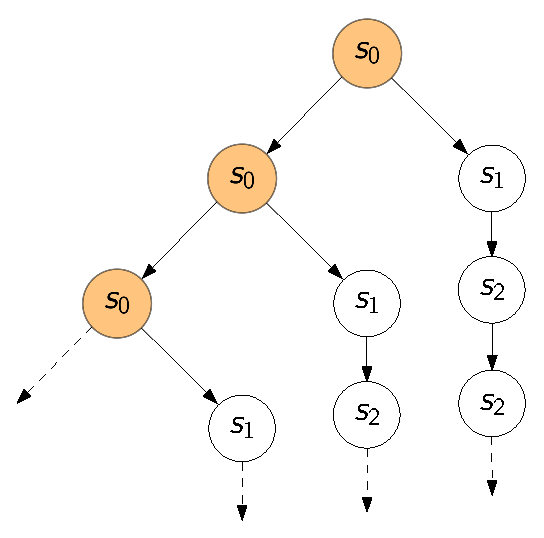
\includegraphics[width=0.6\linewidth]{resources/CTL_counter_example_unfolding}
\end{column}
\begin{column}{0.5\linewidth}
  Le chemin {\color{fibeamer@orange}\[s_0^*s_1s_2^\omega\]} passe par un état $\neg a$ \\(i.e., par $s_1$).
\end{column}
\end{columns}
\vspace{0.01\linewidth}
\begin{itemize}
  \item[$\rightarrow$] Il n'existe pas d'états dans le chemin $s_0^\omega$ qui va satisfaire $\forall \Box a$ car $s_0 \not \models \forall \Box a$
  %\item[$\implies$] $s_0 \not \models \forall \Diamond \forall \Box a$
\end{itemize}
\end{frame}


\section{PCTL}
\subsection{MC}
\begin{frame}
  \small
  \begin{definition}[Chaîne de Markov à temps discret]
  	Une \textit{chaîne de Markov à temps discret}, notée \textbf{MC} (pour \textit{Markov Chain}), est un modèle probabiliste défini par un tuple  $\mathcal{M} = (S, \Delta, AP, L)$ où :
  	\begin{itemize}
  		\item $S$ est un ensemble dénombrable d'états,
  		\item $\Delta: S \times S \rightarrow [0,1] \cap \mathbb{Q}$ est une \textit{fonction de transition} telle que \[\forall s \in S, \sum_{s' \in S}\Delta(s, s')= 1\]
  		%\item $d_0:S \rightarrow [0,1]$ est la distribution initiale telle que \[\sum_{s \in S}d_0(s)= 1\] (à noter que dans le cadre de ce document, la distribution initiale peut être omise, et dans ce cas, $\forall s \in S, d_0(s) = \frac{1}{|S|}$).
  		où $\Delta(s, s')$ est la probabilité de passer de l'état $s$ à l'état $s'$,
      \item $AP$ est un ensemble de propositions atomiques et
      \item $L: S \rightarrow 2^{AP}$ est une fonction d'étiquetage.
  	\end{itemize}
  \end{definition}
\end{frame}

\begin{frame}{Chaînes de Markov}
  \normalsize
  \begin{itemize}
    \item Les MCs sont des modèles \textbf{\color{fibeamer@orange}déterministes}
    \item L'idée des chemins d'une MC est la même que pour les TSs :
  \end{itemize}
  \begin{definition}[Chemin dans une MC]
      Un {\color{fibeamer@orange}chemin} (infini) $\pi = s_0 s_1 s_2 \dots \in S^\omega$ est une séquence d'états de la MC
      $\mathcal{M} = (S, \Delta, AP, L)$ où $\forall i \in \mathbb{N}$, $\Delta(s_i, s_{i+1}) > 0$. \\
      $Paths(s)$ est l'ensemble des chemins de $\mathcal{M}$ qui commencent
      en l'état $s \in S$.
  \end{definition}
\end{frame}
\normalsize
\subsection{Intuition}
\begin{frame}{Logique en arbre de calculs probabiliste (PCTL)}
  \begin{itemize}
    \item CTL probabiliste
    \item Logique temporelle en branchements pour exprimer les {\color{fibeamer@orange}propriétés d'états} des MCs.
    \item Logique proche de CTL pour les systèmes probabilistes.
  \end{itemize}
\end{frame}

\begin{frame}{CTL vs PCTL}
\begin{itemize}
  \item \textbf{\color{fibeamer@orange}CTL :} \\
  Chemins quantifiés en utilisant $\forall$ et $\exists$
  \item \textbf{\color{fibeamer@orange}PCTL :} \\
  Chemins quantifiés en utilisant leur probabilité, avec $\mathcal{P}_J(\phi)$ où $J \subseteq [0, 1]$ et $\phi$ est une formule de chemin
\end{itemize}
\[ s \models \mathcal{P}_J(\phi) \text{ ssi } \mathbb{P}_s(\{\pi \in Paths(s) \; | \; \pi \models \phi \}) \in J\]
  \begin{itemize}
    \item[+] PCTL inclus additionnellement le \textit{until borné} $U^{\leq n}$
  \end{itemize}
\end{frame}

\subsection{Syntaxe}
\begin{frame}{}
  \begin{block}{Syntaxe}
    Soit $AP$, un ensemble de propositions atomiques.
    \begin{itemize}
      \item Les \textit{\color{fibeamer@orange}formules d'états} PCTL sont formées selon la
    grammaire suivante :
    \[
      \Phi ::= true \; | \; a \; | \; \Phi \wedge \Psi \; | \; \neg \Phi \; | \; \mathcal{P}_J(\phi)
    \]
    où $a \in AP$, $J \subseteq [0, 1]$ et $\phi$ est une formule de chemin.
      \item Les \textit{\color{fibeamer@orange}formules de chemins} PCTL sont formées selon la grammaire suivante :
      \[
        \phi ::= \bigcirc\,\Phi \; | \; \Phi U \Psi \; | \; \Phi U^{\leq n} \Psi
      \]
      où $\Phi$ et $\Psi$ sont des formules d'états et $n \in \mathbb{N}$.
    \end{itemize}
  \end{block}
\end{frame}

\subsection{Sémantique}
\begin{frame}{Sémantique}
  Soient $\mathcal{M} = (S, A, \Delta, AP, L)$, une MC et $s \in S$, un {\color{fibeamer@orange}état}
  de $\mathcal{M}$. \\
  $s \models \Phi$ ssi la formule $\Phi$ tient dans l'état $s$, i.e.,
  \begin{align*}
    &s \models true &&&\\
    &s \models a &\text{ ssi }& a \text{ est un label de $s$, i.e., } a \in L(s)&\\
    &s \models \Phi \wedge \Psi&\text{ ssi }& s \models \Phi \text{ et } s \models \Psi&\\
    &s \models \neg \Phi &\text{ ssi }& s \not\models \Phi&\\
    &s \models \mathcal{P}_J(\phi) &\text{ ssi }& \mathbb{P}_s(\phi) \in J&\\
  \end{align*}

    \vspace{-0.05\linewidth}

    où $\mathbb{P}_s(\phi) = \mathbb{P}_s(\{\pi \in Paths(s) \; | \; \pi \models \phi\})$ et $\mathbb{P}_s$ est la mesure de probabilité sur le $\sigma$-algèbre dont les résultats sont les chemins commençant en $s$, i.e.,
    $Paths(s)$
\end{frame}

\begin{frame}{Sémantique}
  Soient $\mathcal{M} = (S, A, \Delta, AP, L)$, une MC et $\pi = s_0s_1s_2\dots \in Paths(s)$, un {\color{fibeamer@orange}chemin}.\\
  $\pi \models \phi$ ssi $\pi$ satisfait $\phi$, i.e.,
  \begin{align*}
  &\pi \models \Phi&\text{ ssi }&s_0 \models \Phi&\\
  &\pi \models \bigcirc\, \Phi&\text{ ssi }&s_1 \models \Phi&\\
  &\pi \models \Phi U \Psi &\text{ ssi }& \exists j \in \mathbb{N},\, s_j \models \Psi
    \text{ et } \forall 0 \leq i < j, \, s_i \models \Phi&\\
  &\pi \models \Phi U^{\leq n} \Psi &\text{ ssi }& \exists 0 \leq j \leq n ,\, s_j \models \Psi
    \text{ et } \forall 0 \leq i < j, \, s_i \models \Phi&\\
  & \pi \models \Diamond \Phi&\text{ ssi }& \exists j \in \mathbb{N}, \, s_j \models \Phi&\\
  & \pi \models \Box \Phi&\text{ ssi }& \forall j \in \mathbb{N}, \, s_j \models \Phi&
  \end{align*}
\end{frame}

\begin{frame}{Sémantique}{Remarque}
  Soient $\mathcal{M} = (S, \Delta, AP, L)$, une MC et $T \subseteq S$, un sous-ensemble d'états de $\mathcal{M}$. \\
  La pseudo-formule de chemin $\Diamond T$ est équivalente à la formule de chemin $\Diamond \Phi$ telle que :
  \begin{itemize}
    \item $\exists T_{AP} \subseteq AP$
    \item $\Phi ::= \bigwedge_{a \in T_{AP}} a$
    \item $\forall t \in T$, $\forall a \in T_{AP}$, $a \in L(t)$
    \item $\forall s \not \in T$, $\exists b \in T_{AP}$ telle que $b \not \in L(s)$
  \end{itemize}
\end{frame}

\begin{frame}{Satisfiabilité}
  L'ensemble de satisfaction d'une MC est essentiellement défini de la même façon que pour les TSs.
  \begin{definition}[Ensemble de satisfaction]
    Soient $\mathcal{M} = (S, A, \Delta, AP, L)$, une MC et
    $\Phi$, une formule d'état PCTL sur $AP$. L'ensemble
    de satisfaction de la MC $\mathcal{M}$ est donné par
    \[
      Sat_\mathcal{M}(\Phi) = \{s \in S \; | \; s \models \Phi \}
    \]
  \end{definition}
\end{frame}

\subsection{Comparaison de logiques temporelles en branchements}
\begin{frame}{PCTL vs CTL}
\[
  s \models \mathcal{P}_{=1}(\Diamond \Phi) \quad  \centernot\implies \quad s \models \forall \Diamond \Phi
\]
\alert{La probabilité que tous les chemins satisfassent une formule de chemin PCTL avec une probabilité de 1 ne signifie pas que tous les chemins satisfassent la formule de chemin CTL correspondante !}
\[
  s \models \mathcal{P}_{>0}(\Box \Phi) \quad  \centernot\Longleftarrow \quad s \models \exists \Box \Phi
\]
\alert{Le fait qu'un chemin satisfasse une formule de chemin CTL n'implique pas forcément que la probabilité des chemins satisfaisant la formules PCTL correspondante soit non-nulle !}
\end{frame}

\begin{frame}{PCTL vs CTL}{Exemple}
  \begin{center}
    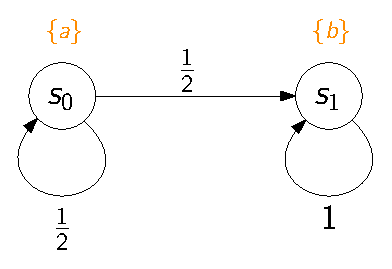
\includegraphics[width=0.5\linewidth]{resources/PCTL_CTL}
  \end{center}
  \begin{itemize}
    \item $s_0 \models \mathcal{P}_{=1}(\Diamond b)$, mais $s \not \models \forall \Diamond b$
    \item $s_0 \models \exists \Box a$, mais $s \not \models \mathcal{P}_{>0}(\Box a)$
  \end{itemize}
\end{frame}

\section{PRCTL}
\subsection{WMC}
\begin{frame}{Chaînes de Markov pondérées}
  \begin{definition}[Chaîne de Markov pondérée]
    Une \textit{chaîne de Markov pondérée} (WMC, pour \textit{weighted Markov chain}) $\mathcal{M}$ est une chaîne de Markov enrichie par une fonction de poids. $\mathcal{M}$ est définie par le tuple $(S, \Delta, AP, L, w)$
    tel que :
    \begin{itemize}
      \item $S, \Delta, AP$ et $L$ sont définis comme pour une MC classique et
      \item $w : S \times S \rightarrow \mathbb{N}^{>0}$ est la fonction
        de poids associant à chaque transition un coût strictement positif.
    \end{itemize}
  \end{definition}
\end{frame}

\begin{frame}{Chaînes de Markov pondérées}{Exemple}
\begin{figure}
  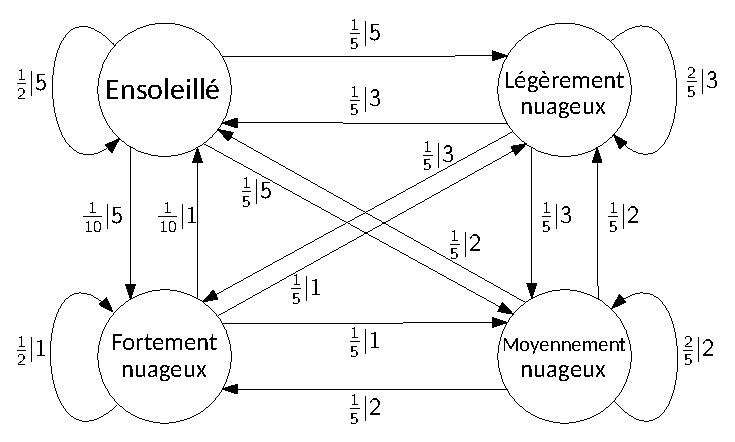
\includegraphics[width=0.8\linewidth]{resources/weather}
  \caption{Système équipé de panneaux solaires produisant de l'énergie en fonction du climat.}
\end{figure}
\end{frame}

\begin{frame}{Chaînes de Markov pondérées}
    Soient $\mathcal{M} = (S, \Delta, AP, L, w)$, une WMC, $s \in S$, un état
    de $\mathcal{M}$, $T \subseteq S$, un sous-ensemble d'états cibles et $\pi \in Paths(s)$.
  \begin{itemize}
  \item $TS^T(\pi)$, la \textit{\color{fibeamer@orange}somme tronquée de $\pi$}, est le coût du chemin $\pi$ jusqu'à satisfaire {(pour la première fois)} $\Diamond T$
  \item $\mathbb{E}_s(TS^T) = \mathbb{E}_s(\{ TS^T(\pi) \; | \; \pi \in Paths(s)  \})$ est l'espérance de la longueur des chemins (en terme de coût) pour que $s \models \mathcal{P}_{=1}(\Diamond T)$ (pour la première fois)
  \item $\mathbb{P}_s(\Diamond_{\leq l}T) = \mathbb{P}_s(\{ \pi \in Paths(s) \; | \; TS^T(\pi) \leq l \})$ est la probabilité que les chemins $\pi_{\in Paths(s)} \models \Diamond T$ avec un coût (i.e., une somme tronquée) inférieure à $l \in \mathbb{N}$.
  \end{itemize}
\end{frame}

\begin{frame}{Chaînes de Markov pondérées}{Exemple}
  \begin{columns}
    \begin{column}{0.5\linewidth}
      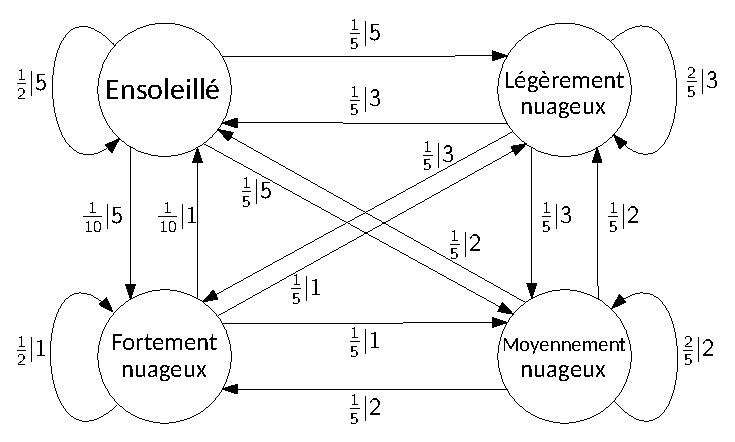
\includegraphics[width=\linewidth]{resources/weather}
    \end{column}
    \begin{column}{0.5\linewidth}
        \begin{align*}
          &TS^{\{Fn\}}(E \cdot Ln \cdot Ln \cdot Mn \cdot Fn\, \dots)& \\
          &= 5+3+3+2 = 13&
        \end{align*}
    \end{column}
  \end{columns}
  \begin{itemize}
    \item $\mathbb{E}_{E}(TS^{\{Fn\}}) = 25 Kj$
    \item $1 - \mathbb{P}_{E}(\Diamond_{\leq 7}\{Fn\}) =
      \mathbb{P}_{E}(\Diamond_{> 8}\{Fn\}) = 1 - 0.14 = 0.86 $
  \end{itemize}
\end{frame}

\subsection{Intuition}
\begin{frame}{PRCTL}{Intuition}
  \begin{itemize}
    \item PCTL + Espérence des ``rewards'' ($\approx$coûts) des chemins.
    \item Inclus un until borné par le coûts des chemins en terme de somme tronquée.
  \end{itemize}
\end{frame}

\subsection{Syntaxe}
\begin{frame}{}
  \small
  \begin{block}{Syntaxe}
    Soit $AP$, un ensemble de propositions atomiques.
    \begin{itemize}
      \item Les \textit{\color{fibeamer@orange}formules d'états} PRCTL sont formées selon la
    grammaire suivante :
    \[
      \Phi ::= true \; | \; a \; | \; \Phi \wedge \Psi \; | \; \neg \Phi \; | \; \mathcal{P}_J(\phi) \; | \; \mathcal{E}_R (\Phi)
    \]
    où $a \in AP$, $J \subseteq [0, 1]$, $R \in [0, +\infty[ \cap \mathbb{N}$ (bornes d'espérances du coût des chemins) et $\phi$ est une formule de chemin.
      \item Les \textit{\color{fibeamer@orange}formules de chemins} PRCTL sont formées selon la grammaire suivante :
      \[
        \phi ::= \bigcirc\,\Phi \; | \; \Phi U \Psi \; | \; \Phi U^{\leq n} \Psi
        \; | \; \Phi U_{\leq r} \Psi
      \]
      où $\Phi$ et $\Psi$ sont des formules d'états et $n, r \in \mathbb{N}$.
    \end{itemize}
  \end{block}
\end{frame}

\subsection{Sémantique}
\begin{frame}{Sémantique}
\small
Soient $\mathcal{M} = (S, A, \Delta, AP, L)$, une MC, $s \in S$, un {\color{fibeamer@orange}état}
  de $\mathcal{M}$ et $\pi = s_0s_1s_2\dots \in Paths(s)$, un {\color{fibeamer@orange}chemin} de $\mathcal{M}$.\\
La sémantique de PRCTL est la même que celle de PCTL, à l'exception que
\begin{itemize}
  \item $s \models \Phi$ ssi la formule $\Phi$ tient dans l'état $s$, i.e.,
    \begin{align*}
      & s \models \mathcal{E}_R(\Phi) & \text{ ssi } & \mathbb{E}_s(\Diamond \Phi) \in R&
    \end{align*}
  \item $\pi \models \phi$ ssi $\pi$ satisfait $\phi$, i.e.,
  \begin{align*}
  &\pi \models \Phi U_{\leq r} \Psi &\text{ ssi }& \exists j \in \mathbb{N} ,\, s_j \models \Psi
    , \;  \forall 0 \leq i < j, \, s_i \models \Phi \text{ et }&\\
  & & & TS^{Sat_\mathcal{M}(\Psi)}(\pi) \leq r &
  \end{align*}
\end{itemize}
\textit{\color{gray}Note : la définition de l'ensemble de satisfaction d'une WMC PRCTL est identique à celle de PCTL}
\end{frame}

\subsection{MDP et stratégies}
\begin{frame}{Processus Décisionnel de Markov et Stratégie}
  \vspace{-0.05\linewidth}
  \begin{itemize}
    \item Un \textit{\color{fibeamer@blue}processus décisionnel de Markov} (MDP, pour \textit{Markov decision process}) est un modèle probabiliste \textbf{\color{fibeamer@orange}non-déterministe}.
    \item $\mathcal{M} = (S, A, \Delta, AP, L, w)$
    \begin{itemize}
      \item Actions : $A$
      \item Fonction de transition : $\Delta : S \times A \times S \rightarrow [0, 1] \cap \mathbb{Q}$
    \end{itemize}
    \item \textit{\color{fibeamer@blue}Chemins} de $\mathcal{M}$ : $\pi = s_0 \xrightarrow{\alpha_0}s_1\xrightarrow{\alpha_1} s_2\xrightarrow{\alpha_2} s_3 \dots$
      \begin{itemize}
        \item $s_i \xrightarrow{\alpha_i} s_{i+1}$% et $(s_i, \alpha, s_{i+1}) \in \rightarrow$
        pour tout $i \in \mathbb{N}$
        \item $\mathcal{H}(\mathcal{M})$ : histoires de $\mathcal{M}$, i.e., l'ensemble des préfixes des chemins de $\mathcal{M}$
      \end{itemize}
    \item \textit{\color{fibeamer@blue}Stratégies} de $\mathcal{M}$, $\sigma : \mathcal{H}(\mathcal{M}) \rightarrow A$
    \item Les décisions d'un MDP $\mathcal{M}$, régulées par une stratégie
      $\sigma$, induisent une MC $\mathcal{M}^\sigma$
  \end{itemize}
\end{frame}

\begin{frame}{Processus Décisionnel de Markov}{Exemple}
  \footnotesize
      \begin{columns}
        \begin{column}[t]{0.5\textwidth}
          \begin{figure}
            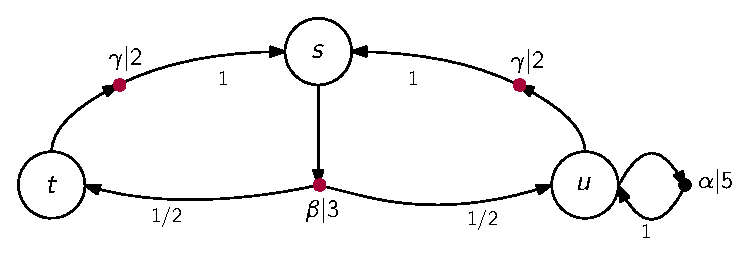
\includegraphics[width=\linewidth]{resources/strat-simple-pdm}
          \end{figure}
        \end{column}
        \begin{column}[t]{0.5\textwidth}
          \begin{itemize}
            \item $\mathcal{M} = (S, A, \Delta, w)$
            \item {\color{fibeamer@orange}$\sigma$}$: S \rightarrow A$,
            \begin{itemize}
              \item {\color{fibeamer@orange}$\sigma$}$(s)=\beta$
              \item {\color{fibeamer@orange}$\sigma$}$(t)=${\color{fibeamer@orange}$\sigma$}$(u) = \gamma$
            \end{itemize}
          \end{itemize}
        \end{column}
      \end{columns}
        \begin{figure}
          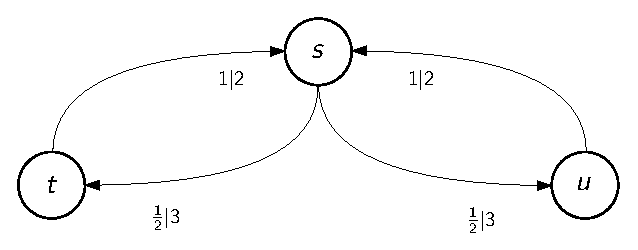
\includegraphics[width=0.5\textwidth]{resources/inducted-markov1}
        \end{figure}
      \begin{center}
    	$ \pi = s \xrightarrow{\beta} t \xrightarrow{\gamma} s \xrightarrow{\beta} u \xrightarrow{\gamma}\dots \in Paths(s)$ \\
        $\pi = s\,t\,s\,u\,{\dots} \in Paths(s)$ est un chemin de {\color{fibeamer@orange}$\mathcal{M}^\sigma$}
      \end{center}
\end{frame}

\begin{frame}{Processus Décisionnel de Markov}
    Soient $\mathcal{M} = (S, A, \Delta, AP, L, w)$, un MDP, $s \in S$, un état
    de $\mathcal{M}$ et $T \subseteq S$, un sous-ensemble d'états cibles.
\begin{itemize}
  \item {\color{fibeamer@blue}$\mathbb{E}_s^{\min}(\Diamond T)$ est l'espérance minimale de la longueur des chemins commençant en $s$ (en terme de somme tronquée) de $\mathcal{M}$}
  \begin{itemize}
    \item i.e., l'espérance de la longueur des chemins commençant en $s$ dans la MC induite par la {\color{fibeamer@orange}stratégie qui minimise l'espérance de la longueur des chemins de $\mathcal{M}$}.
  \end{itemize}
  \item {\color{fibeamer@blue}$\mathbb{P}_s^{\max}(\Diamond_{\leq l} T)$ est la probabilité maximale d'atteindre $T$ depuis $s$ avec un coût inférieur à $l$ dans $\mathcal{M}$}
  \begin{itemize}
    \item i.e., la probabilité d'atteindre $T$ avec un coût inférieure à $l$ dans la MC induite par la {\color{fibeamer@orange}stratégie qui maximise cette probabilité dans $\mathcal{M}$}.
  \end{itemize}
\end{itemize}
\end{frame}

\subsection{PRCTL pour les MDPs}
\begin{frame}{PRCTL pour les MDPs}
  Pour se référer aux MCs induites par ces stratégies, la syntaxe de PRCTL est essentiellement identique, à l'exception des formules d'états suivantes :
  \begin{itemize}
    \item On ne parle plus de $\mathcal{P}_J(\phi)$, mais plutot de $\mathcal{P}_J^{\max}(\phi)$
    \item On ne parle plus de $\mathcal{E}_R(\phi)$, mais plutot de $\mathcal{E}_R^{\min}(\phi)$
  \end{itemize}
    où $J \subseteq [0, 1]$, $R \in [0, +\infty[ \cap \mathbb{N}$ et $\phi$ est une formule de chemin.
\end{frame}

\subsection{PRCTL dans Storm}
\begin{frame}{PRCTL dans Storm}{Exemple}
\begin{columns}
  \begin{column}{0.35\linewidth}
\lstinputlisting[language={Prism},
    numbers=left,
    rulesepcolor=\color{black}, rulecolor=\color{black}, breaklines=true,
    breakatwhitespace=true, firstnumber=1, firstline=1, lastline=25]{resources/simple_mdp.prism}
  \end{column}
  \begin{column}{0.65\linewidth}
    \begin{center}
      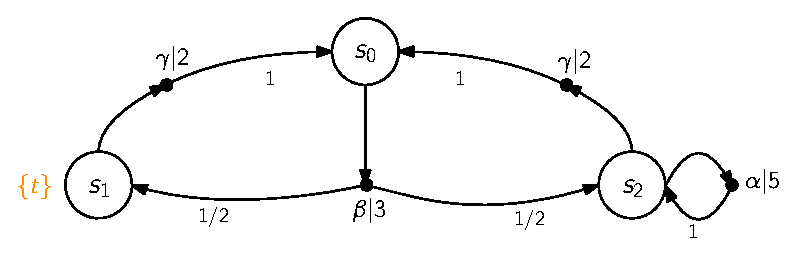
\includegraphics[width=\linewidth]{resources/simple_mdp}
    \end{center}
  \end{column}
\end{columns}
\end{frame}

\begin{frame}[fragile]{PRCTL dans Storm}{Exemple}
%  \begin{center}
%    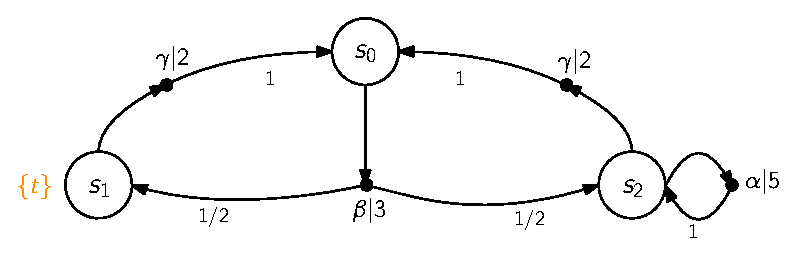
\includegraphics[width=0.65\linewidth]{resources/simple_mdp}
%  \end{center}
\vspace{-0.05\linewidth}
  \[
    s_0 \models \mathcal{E}_{\leq 10}^{\min}(\Diamond t)
  \]
  {\tiny
  \begin{verbatim}
>> storm --prism resources/simple_mdp.prism --prop "Rmin<=10 [F \"t\"]"

Storm 1.2.0

--------------------------------------------------------------
Model type: 	MDP (sparse)
States: 	3
Transitions: 	5
Choices: 	4
Reward Models:  weights
State Labels: 	3 labels
   * deadlock -> 0 item(s)
   * init -> 1 item(s)
   * t -> 1 item(s)
Choice Labels: 	none
--------------------------------------------------------------

Model checking property R[exp]min<=10 [F "t"] ...
Result (for initial states): true

Time for model checking: 0.008s.
  \end{verbatim}
  }
\end{frame}

\begin{frame}[fragile]{PRCTL dans Storm}{Exemple (requête)}
%  \begin{center}
%    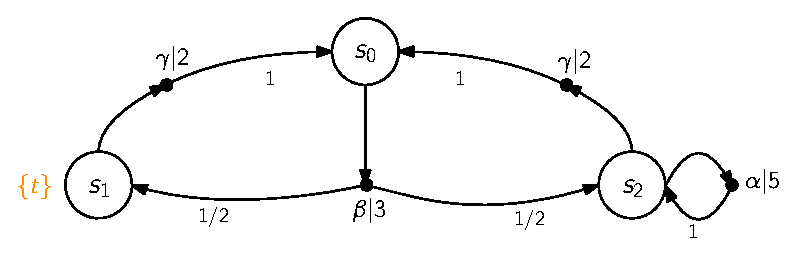
\includegraphics[width=0.65\linewidth]{resources/simple_mdp}
%  \end{center}
\vspace{-0.05\linewidth}
  \[
    s_0 \models \mathcal{E}_{=?}^{\min}(\Diamond t)
  \]
  {\tiny
  \begin{verbatim}
>> storm --prism resources/simple_mdp.prism --prop "Rmin=? [F \"t\"]"

Storm 1.2.0

--------------------------------------------------------------
Model type: 	MDP (sparse)
States: 	3
Transitions: 	5
Choices: 	4
Reward Models:  weights
State Labels: 	3 labels
   * deadlock -> 0 item(s)
   * init -> 1 item(s)
   * t -> 1 item(s)
Choice Labels: 	none
--------------------------------------------------------------

Model checking property R[exp]min=? [F "t"] ...
Result (for initial states): 8
Time for model checking: 0.007s.
  \end{verbatim}
  }
\end{frame}

\begin{frame}[fragile]{PRCTL dans Storm}{Exemple}
%  \begin{center}
%    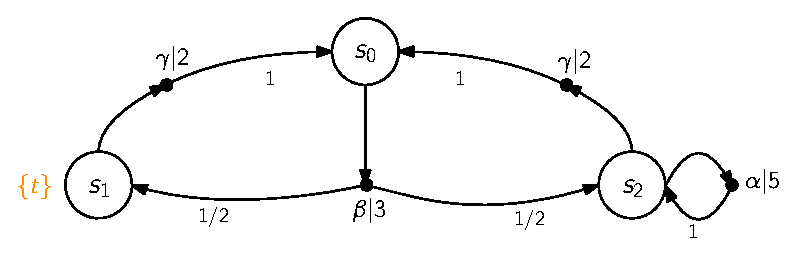
\includegraphics[width=0.65\linewidth]{resources/simple_mdp}
%  \end{center}
\vspace{-0.05\linewidth}
  \[
    s_0 \models \mathcal{P}_{\geq 0.7}^{\max}(\Diamond_{\leq 8} t)
  \]
  {\tiny
  \begin{verbatim}
>> storm --prism resources/simple_mdp.prism --prop "Pmax>=0.7 [F{\"weights\"}<=8 \"t\"]"

Model checking property Pmax>=7/10 [true Urew{"weights"}<=8 "t"] ...
Result (for initial states): true
Time for model checking: 0.000s.
  \end{verbatim}
  }
  \[
    s_0 \models \mathcal{P}_{=?}^{\max}(\Diamond_{\leq 8} t)
  \]
  {\tiny
  \begin{verbatim}
>> storm --prism resources/simple_mdp.prism --prop "Pmax=? [F{\"weights\"}<=8 \"t\"]"

Model checking property Pmax=? [true Urew{"weights"}<=8 "t"] ...
Result (for initial states): 0.75
Time for model checking: 0.010s.s.
  \end{verbatim}
  }
\end{frame}

\subsection{}
\begin{frame}[allowframebreaks]
        \frametitle{References}
      \printbibliography
\end{frame}

\end{document}
